% !TeX document-id = {1e557515-5bd4-45c0-acc0-efd3f93a342d}
% !TeX TXS-program:compile = txs:///pdflatex/[--shell-escape]
\documentclass[]{scrreprt}


\usepackage[swedish,english]{babel}
\usepackage[utf8]{inputenc}
\usepackage{minted}
\usepackage{graphicx}
% roman numeral
\newcommand{\RN}[1]{%
	\textup{\uppercase\expandafter{\romannumeral#1}}%
}

% Title Page
\title{Game Of Life}
\author{Gardström Emil \and Wallin Dennis}
\subtitle{Beräkningsvetenskap \RN{1}}
\titlehead{\Large Uppsala Universitet\hfill KandMa}


\begin{document}
\maketitle

\selectlanguage{english}
\begin{abstract}
	The Game of Life was first conceived in 1970 by Conway J.H. This project aims to recreate this simulation of living cells using Matlab. This is done by drawing each generation of the simulation.
\end{abstract}
\selectlanguage{swedish}
\chapter{Inledning}
\section{Situation}
I detta projekt får vi öva på programmering inklusive if-satser, funktioner och loopar.
\section{Problem}
\chapter{Resultat}
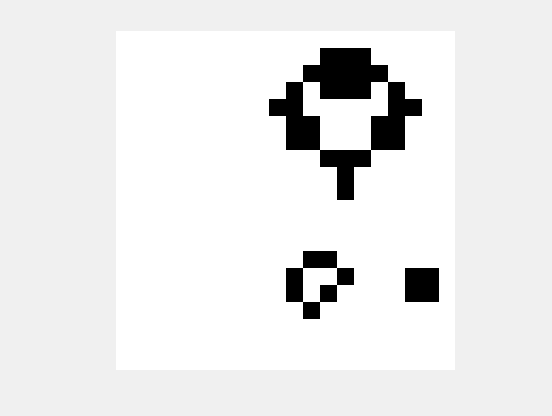
\includegraphics[height=6cm]{src/rendered.png}
\appendix
\chapter{simulate.m}
\inputminted[linenos=true,frame=leftline]{matlab}{src/simulate.m}
%\lstinputlisting[language=matlab,numbers=left,frame=L]{src/simulate.m}
\chapter{gof.m}
\inputminted[linenos=true,,frame=leftline]{matlab}{src/gof.m}
%\lstinputlisting[language=matlab,numbers=left,frame=L]{src/gof.m}
\end{document}     